\subsection{Giới thiệu về vector}
Xét một tình huống mà ở đó bạn di chuyển 3m về phía Bắc, sau đó đi tiếp 4m về phía Đông. Nếu như bạn chỉ quan tâm đến quãng đường mình đã đi được, ta chỉ đơn giản là lấy \(3+4=7\si{m}\). Tuy nhiên, khi ta xét đến \textbf{Độ rời} hay khoảng cách giữ 2 điểm đầu và cuối, kết quả sẽ là \(\sqrt{3^2+4^2}=5\si{m}\). Như vậy, ta có thể thấy rằng việc chỉ xét đến độ dài của đoạn đường là không đủ, mà cần phải xét đến cả phương và chiều của đoạn đường đó.
\begin{figure}[H]
\centering
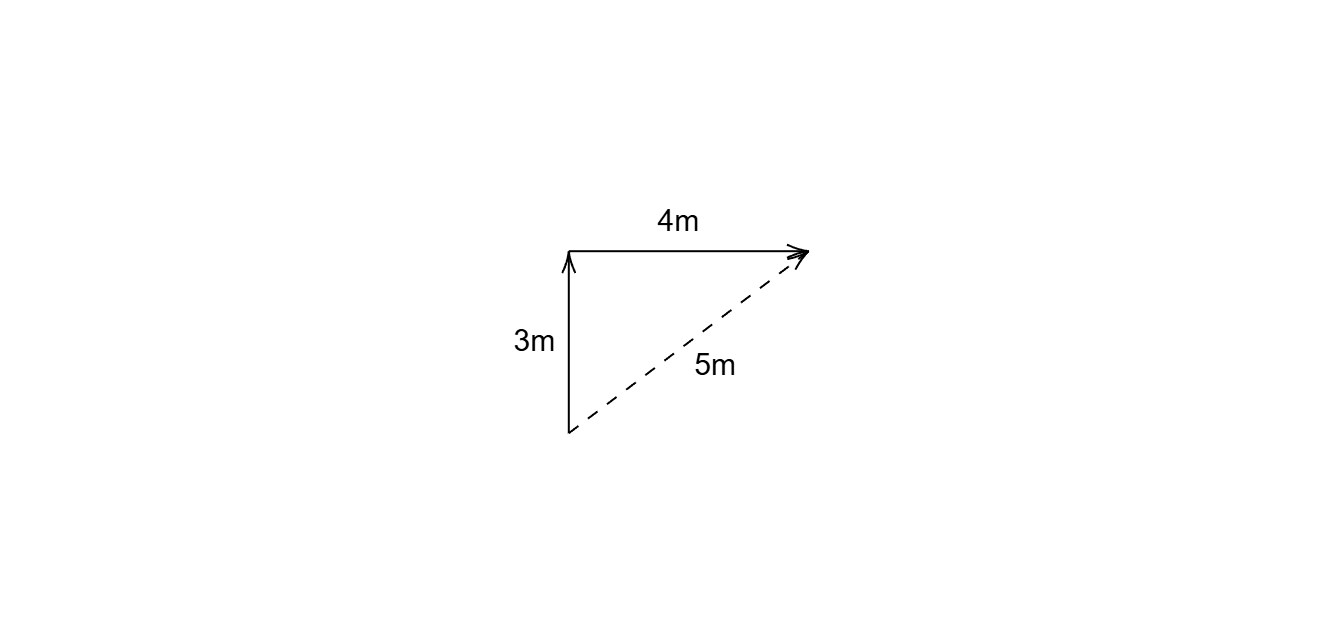
\includegraphics[width=1\textwidth]{Tuan2/Figures/gioithieuvector.png}
\end{figure}
Chúng ta sẽ làm việc với những bài toán như vậy khá nhiều, vì vậy sẽ là cần thiết để định nghĩa một đối tượng toán học có thể mô tả cả độ lớn và hướng. Đối tượng này được gọi là \textbf{vector}.
\begin{definition} Vector \(AB\) (hình vẽ), kí hiệu là \(\overrightarrow{AB}\), là một mũi tên được đặc trưng bởi độ dài \(a\) của nó (do đó còn được kí hiệu là \(\overrightarrow{a}\)) và hướng mà nó chỉ.
\end{definition}
\begin{figure}[H]
\centering

\includegraphics[width=1\textwidth]{Tuan2/Figures/vectorAB.png}
\end{figure}
Như vậy, các đại lượng được có hướng như vận tốc, lực có thể được định nghĩa bởi một vector, còn các đại lượng vô hướng như khôi lượng, nhiệt độ thì không.

Ta sẽ tiếp tục với một số định nghĩa liên quan đến vector.
\begin{definition}
    So sánh hai vector:
    \begin{itemize}
        \item Hai vector \(\overrightarrow{a}\) và \(\overrightarrow{b}\) được coi là bằng nhau nếu chúng có cùng độ dài và cùng hướng, kí hiệu là \(\overrightarrow{a}=\overrightarrow{b}\).
        \item Hai vector \(\overrightarrow{a}\) và \(\overrightarrow{b}\) có cùng phương nếu chúng song song.
        \item Hai vector \(\overrightarrow{a}\) và \(\overrightarrow{b}\) có cùng giá nếu chúng cùng nằm trên một đường thẳng.
    \end{itemize}
\end{definition}
Để hiểu được vì sao vector lại quan trọng, ta sẽ tìm hiểu các phép toán với vector.

\subsection{Các phép toán trên vector}

\subsubsection{Phép cộng vector}
Quay trở lai bài toán ở phần 2.1.1, thay vì cộng độ lớn của hai quãng đường để có được tổng quãng đường đi được, ta sẽ coi hai quãng đường là hai vector và thực hiện phép cộng vector để có được vector độ dịch chuyển từ điểm đầu đến điểm cuối.
\begin{figure}[H]
    \centering
    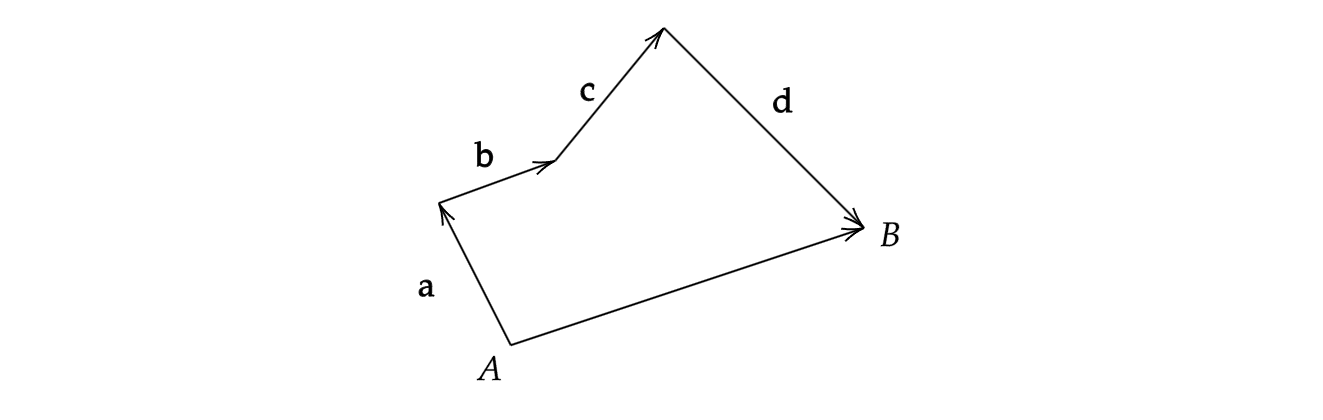
\includegraphics[width=1\textwidth]{Tuan2/Figures/congvector.png}
    \caption{$\overrightarrow{a}+\overrightarrow{b}+\overrightarrow{c}+\overrightarrow{d}=\overrightarrow{AB}$}
\end{figure}

\subsubsection{Tích một vector với một đại lượng vô hướng}
Khi nhân một vector với một đại lượng vô hướng, độ dài của vector sẽ được nhân lên với hệ số bằng đại lượng đó, trong khi hướng của vector không đổi.
\begin{figure}[H]
    \centering
    
\includegraphics[width=1\textwidth]{Tuan2/Figures/vector x vo huong.png}
    \caption{phép nhân vector với một đại lượng vô hướng}
\end{figure}

\subsubsection{Tích vô hướng hai vector}
Phép nhân vô hướng hai vector \(\overrightarrow{a}\) và \(\overrightarrow{b}\) có kết quả là một đại lượng vô hướng có giá trị bằng:
\begin{equation}
    \overrightarrow{a} \cdot \overrightarrow{b} = |\overrightarrow{a}| |\overrightarrow{b}| \cos (\overrightarrow{a}, \overrightarrow{b})
\end{equation}
Ý nghĩa của phép nhân vô hướng được thể hiện như hình vẽ
\begin{figure}[H]
    \centering
    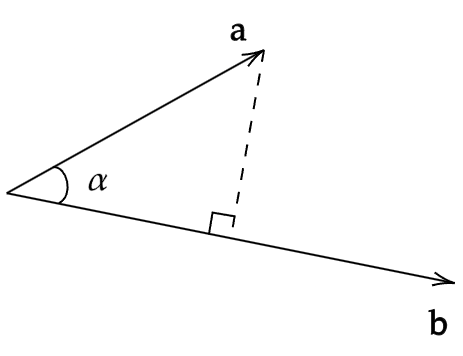
\includegraphics[width=1\textwidth]{Tuan2/Figures/tichcham.png}
    \caption{phép nhân vô hướng hai vector}
\end{figure}
\subsubsection{Tích có hướng hai vector}
Phép nhân có hướng hai vector \(\overrightarrow{a}\) và \(\overrightarrow{b}\) có kết quả là một vector hướng vuông góc với mặt phẳng chứa hai vector này:
\begin{figure}[H]
    \centering
    
\includegraphics[width=1\textwidth]{Tuan2/Figures/tichcheo.png}
    \caption{phép nhân có hướng hai vector}
\end{figure}
Vector này có độ dài bằng:
\begin{equation}
    |\overrightarrow{a} \times \overrightarrow{b}| = |\overrightarrow{a}| |\overrightarrow{b}| \sin (\overrightarrow{a}, \overrightarrow{b})
\end{equation}
Chiều của vector này có thể được xác định bằng quy tắc bàn tay phải, hoặc quy tắc vặn nút chai.

